\documentclass[11pt,oneside]{article}
\input{coursHeadings}

\usepackage[%
    pdftitle={TD Communication technique},
    pdfauthor={Xavier Pessoles},
    colorlinks=true,
    linkcolor=blue,
    citecolor=magenta]{hyperref}



% \makeatletter \let\ps@plain\ps@empty \makeatother
%% DEBUT DU DOCUMENT
%% =================
\sloppy
\hyphenpenalty 10000

\newcommand{\Pointilles}[1][3]{%
\multido{}{#1}{\makebox[\linewidth]{\dotfill}\\[\parskip]
}}


\begin{document}


\newboolean{prof}
\setboolean{prof}{false}
%------------- En tetes et Pieds de Pages ------------
\pagestyle{fancy}
\renewcommand{\headrulewidth}{0pt}

\fancyhead{}
\fancyhead[L]{%
\begin{minipage}[c]{1.6cm}
\includegraphics[width=2cm]{png/logo_ptsi.png}%
\end{minipage}
\rule{2cm}{.5pt}
}

\fancyhead[C]{\rule{11cm}{.5pt}}

\fancyhead[R]{%
\begin{minipage}[c]{3cm}
\begin{flushright}
\footnotesize{\textit{\textsf{Sciences Industrielles\\ pour l'Ingénieur}}}%
\end{flushright}
\end{minipage}
}

\renewcommand{\footrulewidth}{0.2pt}

\fancyfoot[C]{\footnotesize{\bfseries \thepage}}
\fancyfoot[L]{\footnotesize{2012 -- 2013} \\ X. \textsc{Pessoles}}
\ifthenelse{\boolean{prof}}{%
\fancyfoot[R]{\footnotesize{TD -- CI 5 : Communication technique -- P}}
}{%
\fancyfoot[R]{\footnotesize{TD -- CI 5 : Communication technique}}
}


%\begin{center}
%\textit{Centre d'intérêt}
%\end{center}


\begin{center}
 \huge\textsc{CI 5 -- Communication technique}
\end{center}

\begin{center}
 \LARGE\textsc{Représentation des pièces mécaniques}
\end{center}


%\begin{center}
 %\LARGE\textsc{PINCE SCHRADER}
%\end{center}

\vspace{.5cm}

\textit{D'après documents de Jean-Pierre Pupier}

\begin{contexte}
\begin{itemize}
\item Contexte technique : représentation de pièces géométriques diverses
\item Objectifs : 
\begin{itemize}
\item savoir passer d'une représentation 3D à une représentation 2D en respectant les normes de représentation
\end{itemize}
\end{itemize}
\end{contexte}

\section*{Butée réglable}

\begin{enumerate}
\item Complétez les trois vues suivantes.
\item Repassez en couleur les arêtes repérées sur la perspective.
\end{enumerate}

\begin{center}
\includegraphics[width=.6\textwidth]{png/fig1}
\end{center}

\section*{Porte-outil}

\begin{enumerate}
\item Complétez les trois vues suivantes.
%\item Repassez en couleur les arêtes repérées sur la perspective.
\end{enumerate}

\begin{center}
\includegraphics[width=.6\textwidth]{png/fig2}
\end{center}

\newpage
\section*{Palier}

\begin{enumerate}
\item Terminez la vue de face et la vue de gauche en coupe B-B.
\item Terminez la vue de dessus en demi-coupe A-A, la partie coupée étant représentée à droite de l’axe de symétrie vertical.

\end{enumerate}

\begin{center}
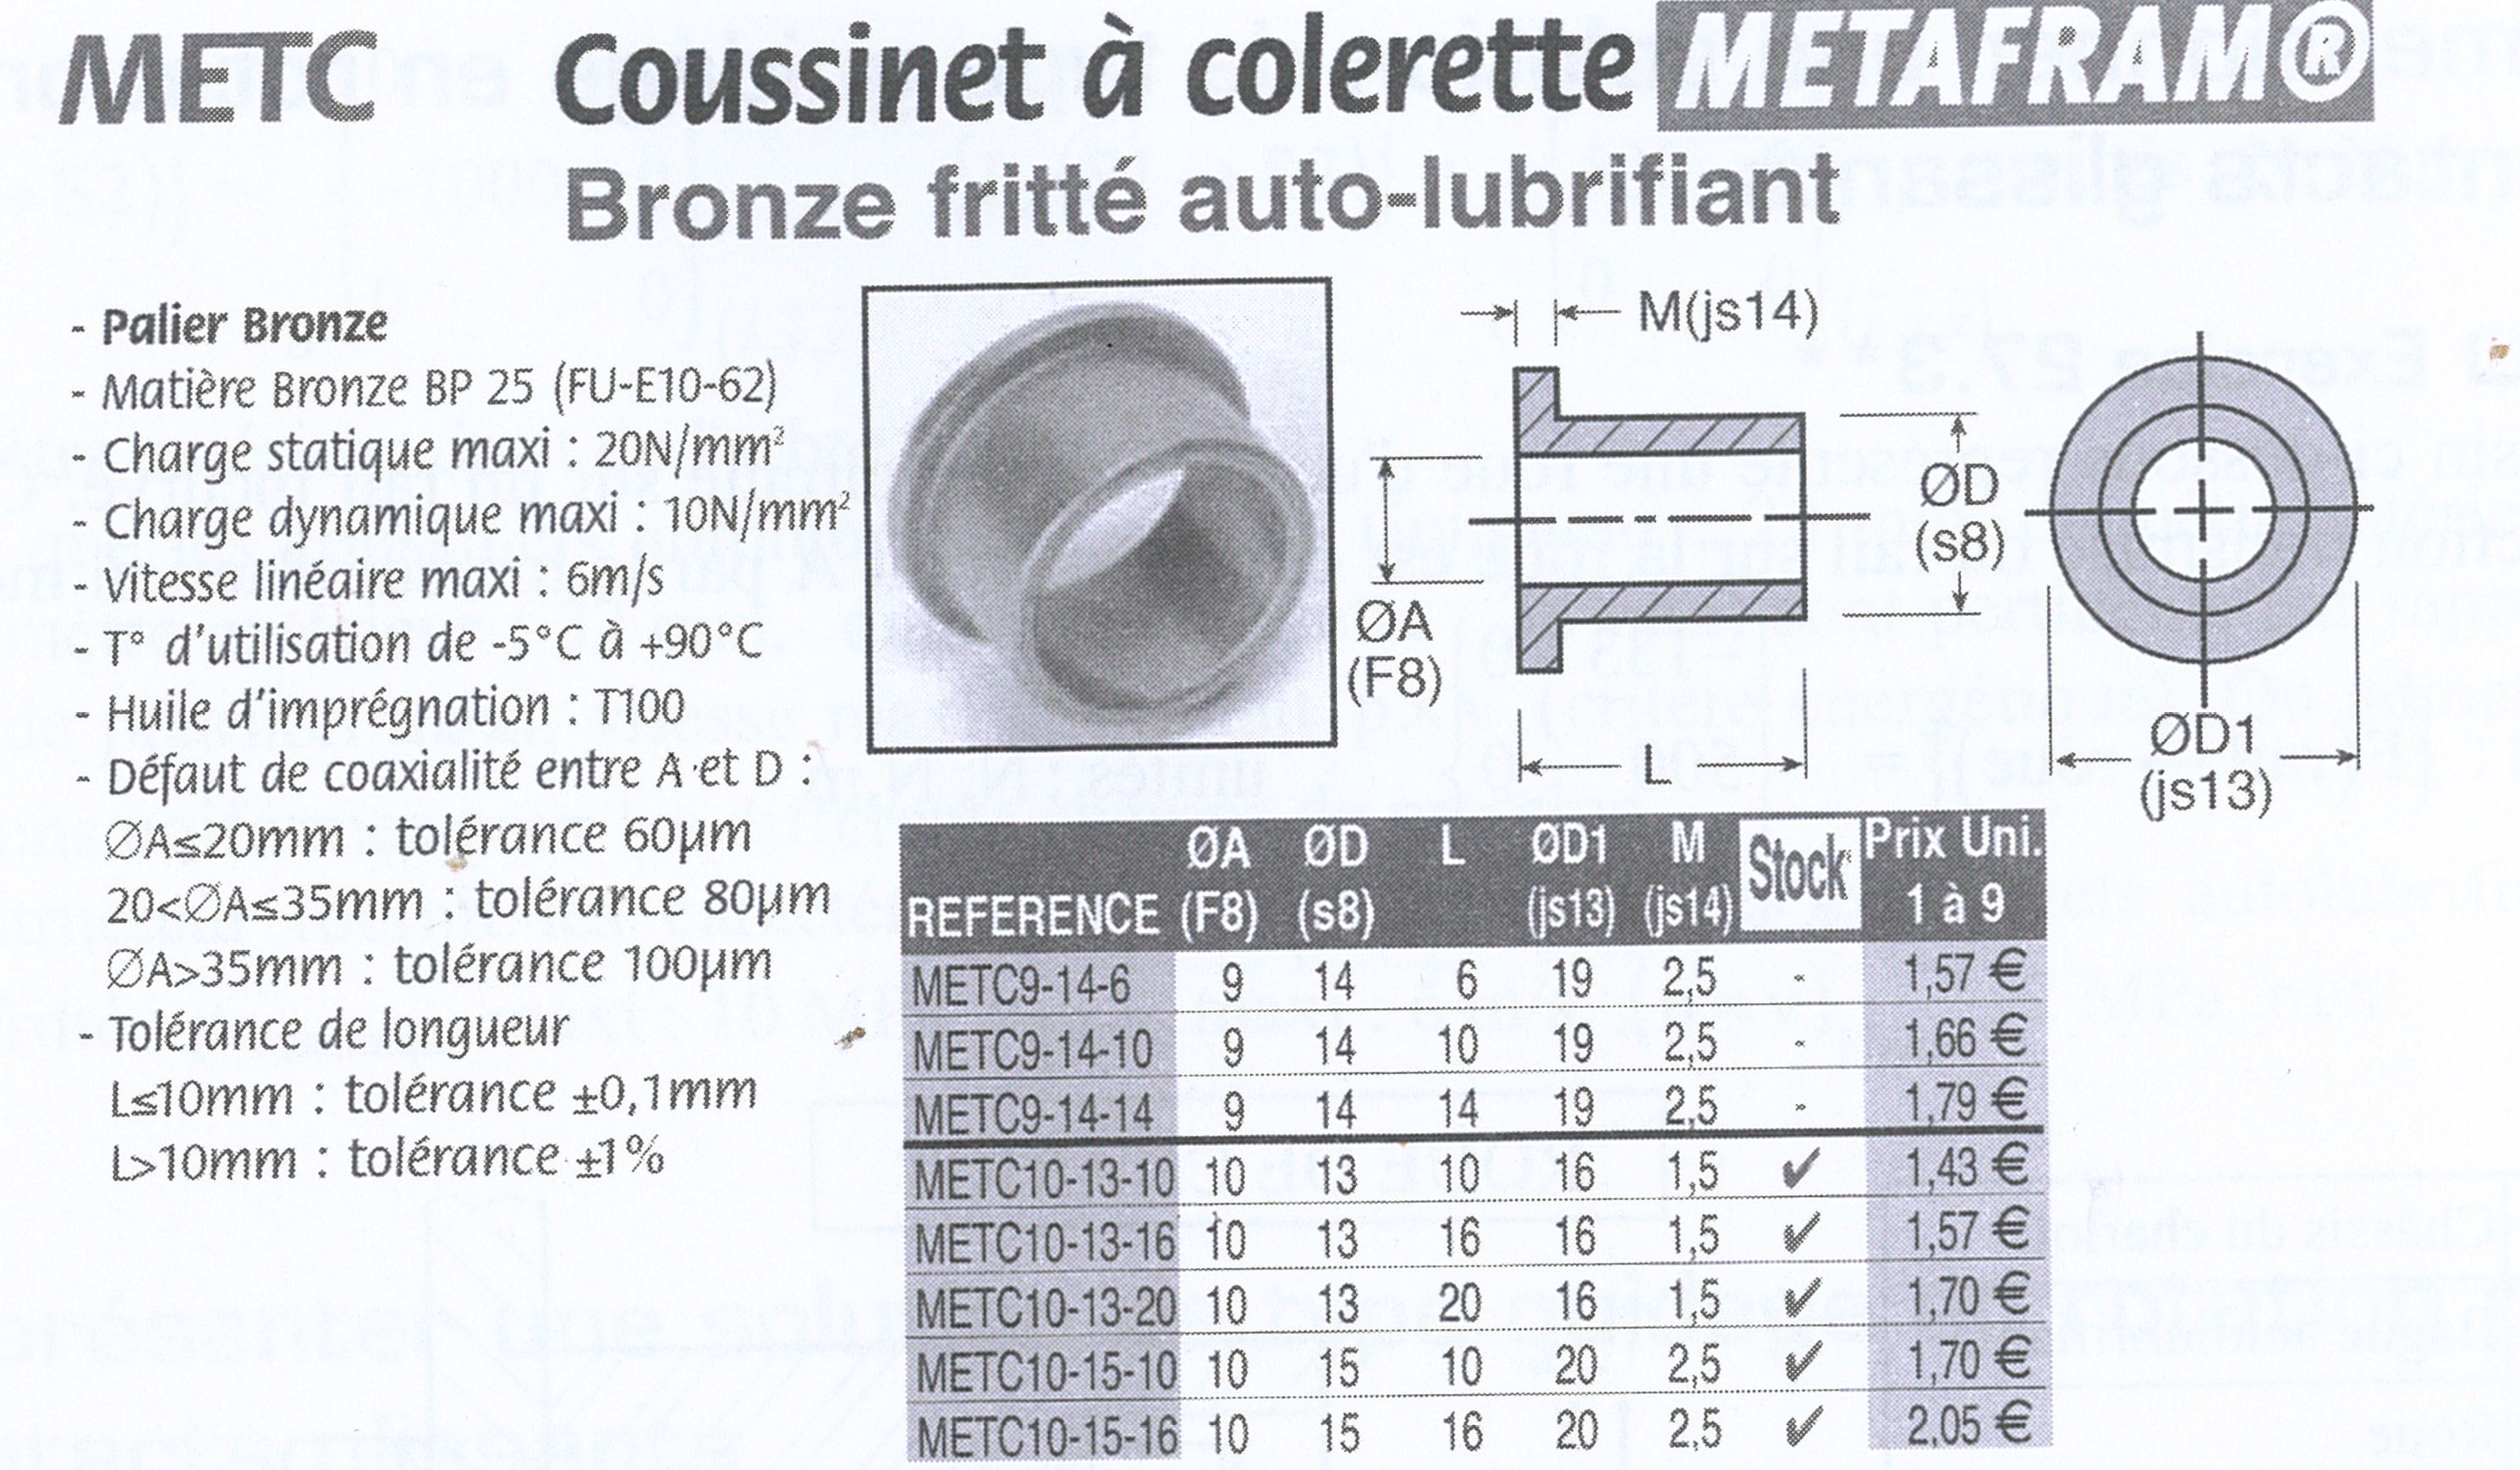
\includegraphics[width=\textwidth]{png/fig3}
\end{center}

\end{document}